\documentclass{TIJMUjiaoanLL}
\pagestyle{empty}


\begin{document}


%课程名称
\kecheng{系统生物学}
%课程内容
\neirong{转录组学(RNA-Seq概述)\ /\ 第3章}
%教师姓名
\jiaoshi{伊现富}
%职称
\zhicheng{讲师}
%教学日期(格式:XXXX年XX月XX日XX时-XX时)
\riqi{2016年9月27日13:30-15:30}
%授课对象(格式:XXX系XXXX年级XX班(硕/本/专科))
\duixiang{生物医学工程与技术学院2013级生信班(本)}
%听课人数
\renshu{28}
%授课方式
\fangshi{理论讲授}
%学时数
\xueshi{2}
%教材版本
\jiaocai{系统生物学,第1版}


%教案首页
\firstHeader
\maketitle
\thispagestyle{empty}

\mudi{
\begin{itemize}
  \item 掌握基因表达谱、转录组学等基本概念,RNA-Seq流程中的关键步骤,RNA-Seq的专用术语。
  \item 熟悉转录组学的研究内容和主要方法,RNA-Seq的常见应用。
  \item 了解常见的组学,RNA-Seq的主要技术。
  \item 自学转录组学研究的其他技术。
\end{itemize}
}

\fenpei{
\begin{itemize}
  \item (5')引言与导入:回顾第二代测序的主要技术和基本流程。
  \item (30')转录组学:介绍常见的组学,讲解转录组学的基本概念和研究内容与方法。
  \item (40')RNA-Seq简介:介绍RNA-Seq,讲解RNA-Seq的主要技术和常见应用。
  \item (20')RNA-Seq流程:介绍RNA-Seq的基本流程,总结实验操作与数据分析的关键步骤,讲解RNA-Seq的专用术语。
  \item (5')总结与答疑:总结授课内容中的知识点与技能,解答学生疑问。
\end{itemize}
}

\zhongdian{
\begin{itemize}
  \item 重点:RNA-Seq流程中的关键步骤,RNA-Seq的专用术语。
  \item 难点:RNA-Seq的专用术语。
  \item 解决策略:通过实例讲解和比较类比帮助学生理解、记忆。
\end{itemize}
}

\waiyu{
  \vspace*{-10pt}
  \begin{multicols}{2}
    基因表达(gene expression)

    基因表达谱(gene expression profile)

    转录组(transcriptome)

    DNA元件百科全书(Encyclopedia of DNA Elements,ENCODE)

    RPKM(Reads Per Kilobase Million)
    
    FPKM(Fragments Per Kilobase Million)

    TPM(Transcripts Per Kilobase Million)
  \end{multicols}
  \vspace*{-10pt}
}

\fuzhu{
\begin{itemize}
  \item 多媒体:常见组学介绍,转录组学的研究方法,RNA-Seq的常见应用。
  \item 板书:RNA-Seq的主要流程,RPKM/FPKM/TPM的计算方法。
\end{itemize}
}

\sikao{
  \vspace*{-10pt}
  \begin{multicols}{2}
  \begin{itemize}
    \item 什么是转录组学?
    \item 总结转录组学的研究内容和方法。
    \item 列举RNA-Seq的常见应用。
    \item 总结RNA-Seq的基本流程。
    \item 解释并计算RPKM/FPKM/TPM。
  \end{itemize}
  \end{multicols}
  \vspace*{-10pt}
}

\cankao{
\begin{itemize}
  \item 维基百科等网络资源。
\end{itemize}
}

\firstTail


%教案续页
\newpage
\otherHeader

\begin{enumerate}
  \item 引言与导入(5分钟)
    \begin{enumerate}
      \item 二代测序技术:Roche/454,Illumina/Solexa,ABI/SOLiD
      \item 二代测序流程:实验流程,分析流程(QC,Mapping,Annotation)
    \end{enumerate}

  \item 转录组学(30分钟)
    \begin{enumerate}
\parpic[fr]{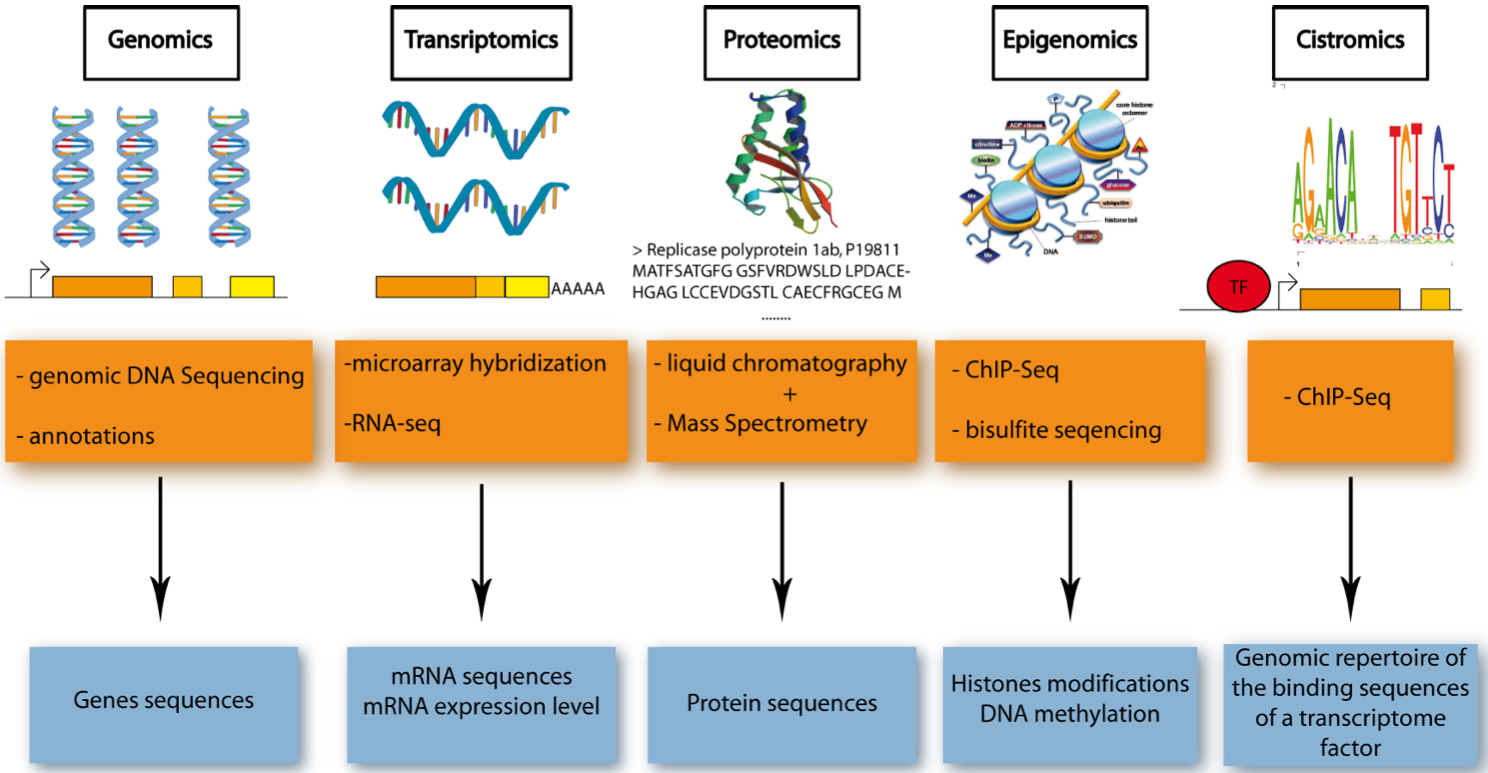
\includegraphics[width=8.8cm]{c3.omics.03.png}}
      \item 组学\textcolor{red}{(结合分子生物学中的中心法则等知识点进行讲解)}
        \begin{itemize}
          \item Genomics $\Leftarrow$ DNA
          \item Transcriptomics $\Leftarrow$ RNA
          \item Proteomics $\Leftarrow$ Protein
          \item Epigenomics $\Leftarrow$ Methylation/Histone
          \item Cistomics $\Leftarrow$ Cistron(DNA-Protein)
          \item Metabolomics $\Leftarrow$ Small molecules
        \end{itemize}
      \item 转录组学
        \begin{enumerate}
          \item 基本概念
            \begin{itemize}
              \item 基因表达:基因中的信息合成基因产物(\textcolor{red}{蛋白质+ RNA})的过程
              \item 基因表达谱:是否表达,表达丰度,表达差异,……
              \item mRNA丰度:每个细胞里每一种mRNA分子的平均数
              \item 转录组
                \begin{itemize}
                  \item 广义:相同环境(或生理条件)下的在一个细胞或一群细胞中所能转录出的所有RNA的总和
                  \item 狭义:细胞所能转录出的所有mRNA
                \end{itemize}
            \end{itemize}
          \item 转录组学\textcolor{red}{(时空的连续性 vs. 快照,动 vs. 静;以电影和截图进行类比)}
            \begin{itemize}
\parpic[fr]{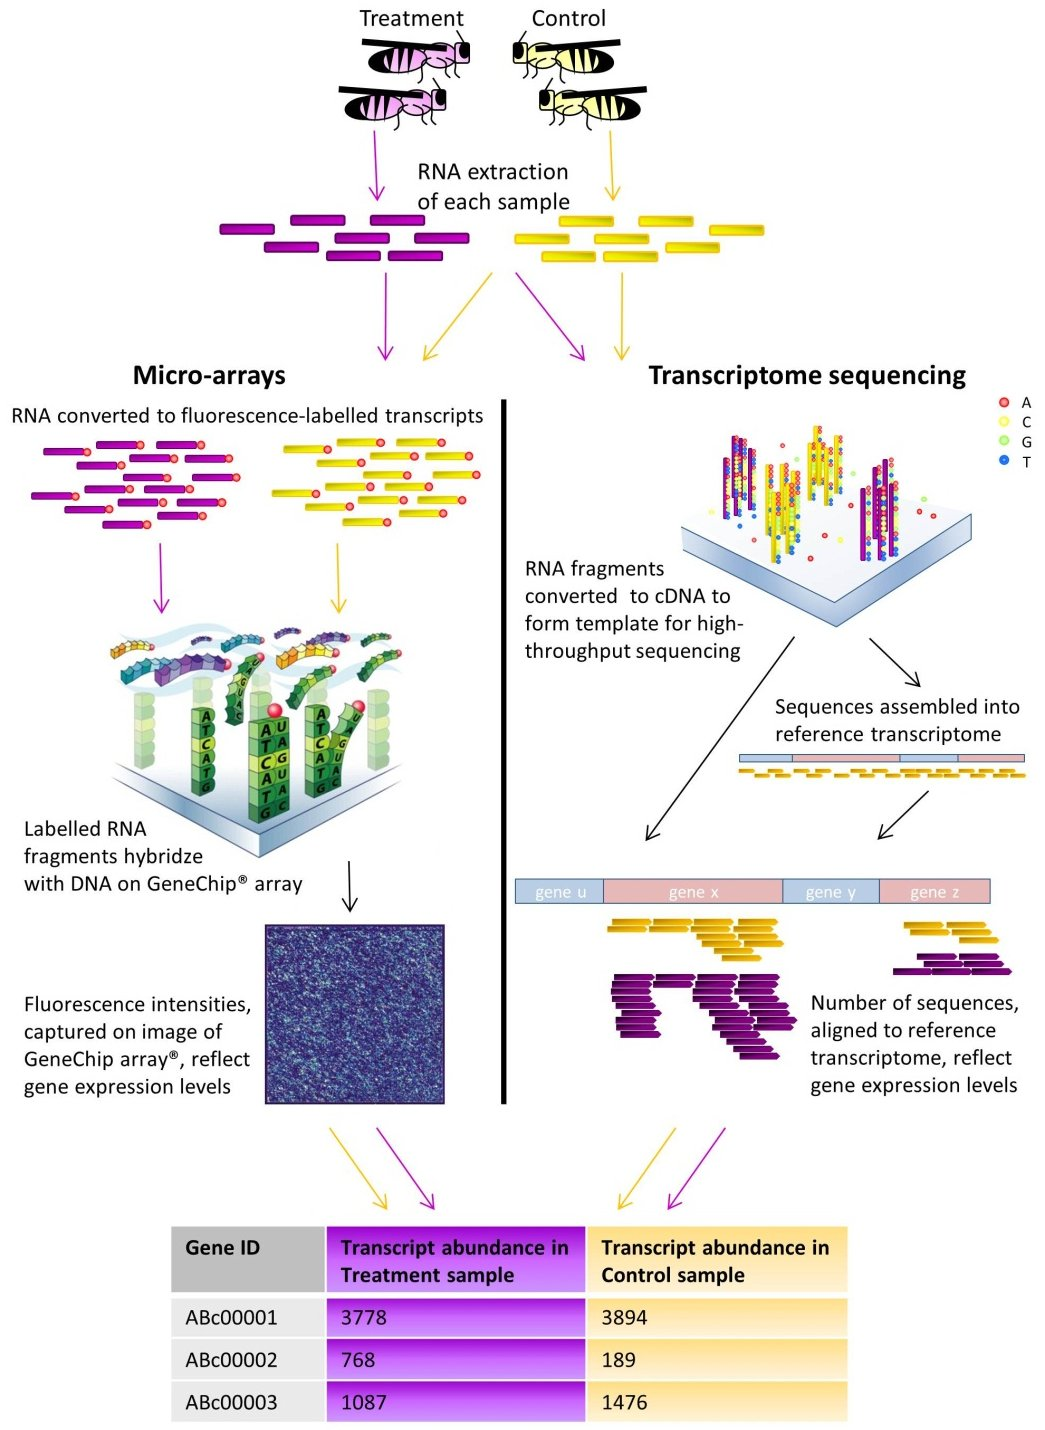
\includegraphics[width=6cm]{c3.trans.method.03.jpg}}
              \item 定义:对转录水平上发生的事件及其相互关系和意义进行整体研究的一门学科
              \item 研究内容
                \begin{itemize}
                  \item 对特定细胞的转录与加工机制进行研究
                  \item 对转录物编制目录便于进一步归类研究
                  \item 绘制动态的转录物图形
                  \item 转录物调控网络
                \end{itemize}
              \item 研究方法\textcolor{red}{(Microarray vs. RNA-Seq)}
                \begin{itemize}
                  \item EST:expressed sequence tag,表达序列标签
                  \item SAGE:serial analysis of gene expression
                  \item MPSS:massive parallel signature sequencing
                  \item Microarray
                  \item RNA-Seq:RNA sequencing
                \end{itemize}
            \end{itemize}
        \end{enumerate}
    \end{enumerate}

  \item RNA-Seq简介(30分钟)
    \begin{enumerate}
      \item 基本概念
        \begin{itemize}
          \item RNA:mRNA(intron, polyA),rRNA+tRNA(95\%),\textcolor{red}{ncRNA}
          \item RNA-Seq:RNA $\Rightarrow$ cDNA $\Rightarrow$ DNA测序
          \item RNA-Seq技术:Poly(A) library, reverse transcription, size selection, ……
        \end{itemize}
      \item 转录本组装\textcolor{red}{(以拼图进行类比)}
        \begin{itemize}
          \item genome-guided:easier, computationally cheaper
          \item \textit{de novo}:difficult
        \end{itemize}

\otherTail
\newpage
\otherHeader

      \item 应用\textcolor{red}{(结合实例进行讲解)}
        \begin{itemize}
          \item Gene expression:Measuring mRNA concentration levels
\parpic[fr]{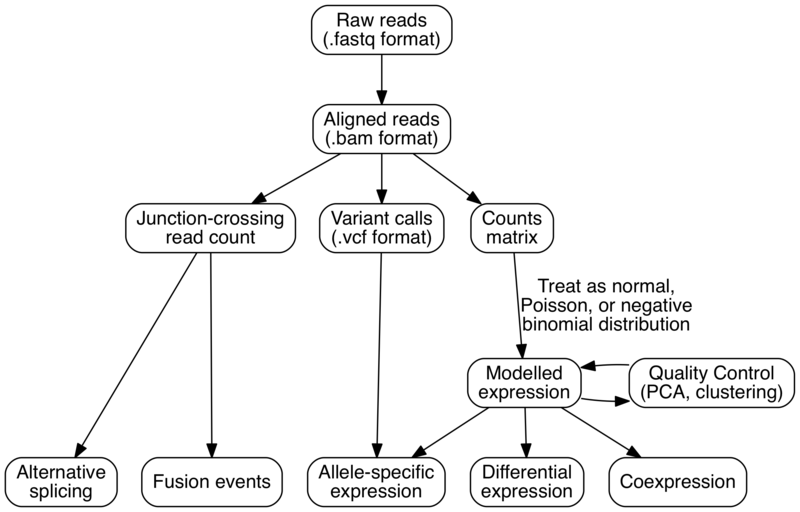
\includegraphics[width=8cm]{c3.rs.analysis.workflow.01.png}}
          \item Differential expression:DGE
          \item Absolute quantification of transcripts
          \item SNV discovery:\textcolor{red}{RNA-Seq vs. DNA-Seq}
          \item Post-transcriptional edits
          \item Fusion gene detection
          \item Alternative transcript usage
          \item Coexpression networks
          \item ……
        \end{itemize}
      \item 数据库
        \begin{itemize}
          \item ENCODE:Encyclopedia of DNA Elements
          \item TCGA:The Cancer Genome Atlas
        \end{itemize}
    \end{enumerate}

  \item RNA-Seq流程(30分钟)
    \begin{enumerate}
      \item \textcolor{red}{【重点】}主要流程\textcolor{red}{(与外显子组测序进行比较)}
        \begin{itemize}
          \item 实验:Purify RNA $\Rightarrow$ Deplete rRNA/Select mRNA $\Rightarrow$ Fragment $\Rightarrow$ cDNA $\Rightarrow$ Add adapter $\Rightarrow$ Size selection $\Rightarrow$ PCR $\Rightarrow$ Sequencing
          \item 分析:QC $\Rightarrow$ Pre-processing $\Rightarrow$ Mapping $\Rightarrow$ Assembly $\Rightarrow$ Counting $\Rightarrow$ Normalizing $\Rightarrow$ DE $\Rightarrow$ Annotation $\Rightarrow$ Vizualization
        \end{itemize}
        \vspace{-1em}
        \begin{figure}[h]
          \centering
          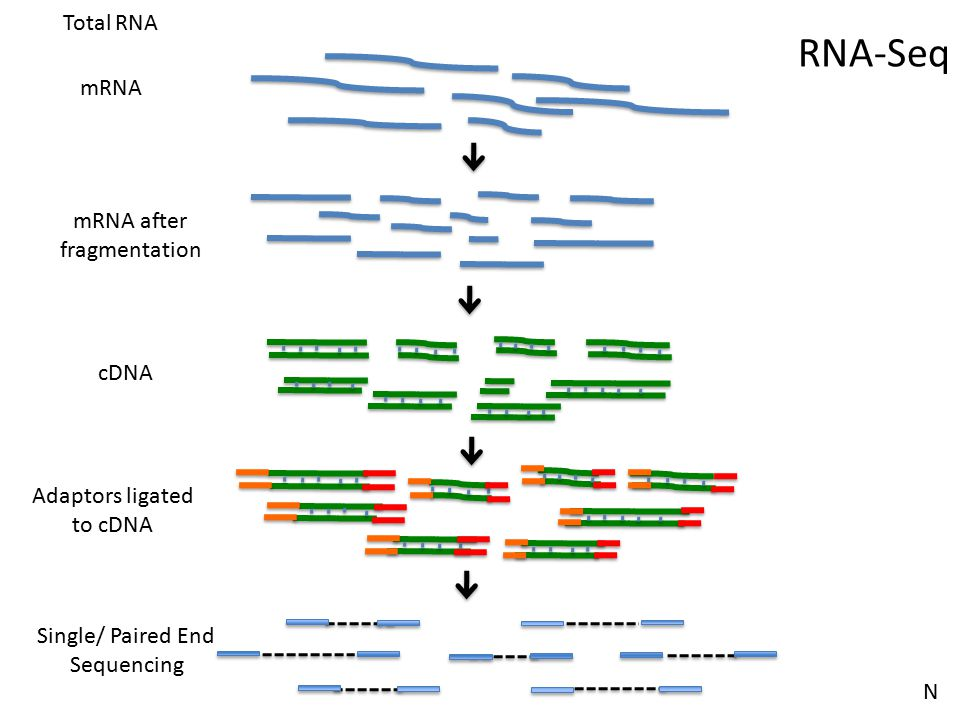
\includegraphics[width=0.45\textwidth]{c3.workflow.exp.11.jpg}
          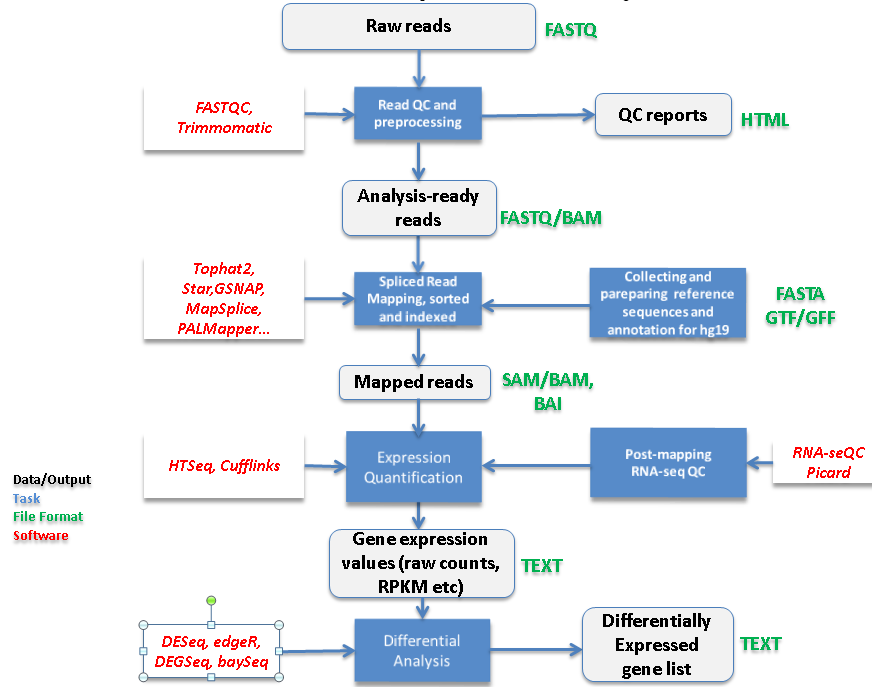
\includegraphics[width=0.45\textwidth]{c3.workflow.tool.format.02.png}
        \end{figure}
        \vspace{-1em}
\parpic[fr]{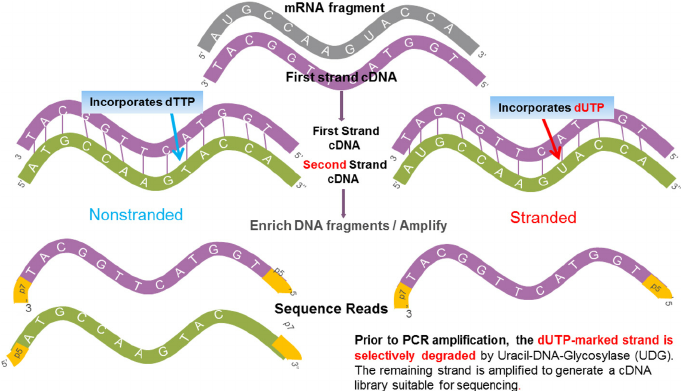
\includegraphics[width=8cm]{c3.workflow.strand.02.png}}
      \item 相关技术
        \begin{itemize}
          \item Single cell RNA sequencing
          \item Stranded sequencing
          \item miRNA sequencing
        \end{itemize}
      \item \textcolor{red}{【重点,难点】}专用术语\textcolor{red}{(通过简单的例子进行概念讲解,并应用公式进行实际演算;强调每种方法的适用范围、优缺点及相互之间的关系)}
        \begin{itemize}
          \item RPKM:Reads Per Kilobase Million
\parpic[fr]{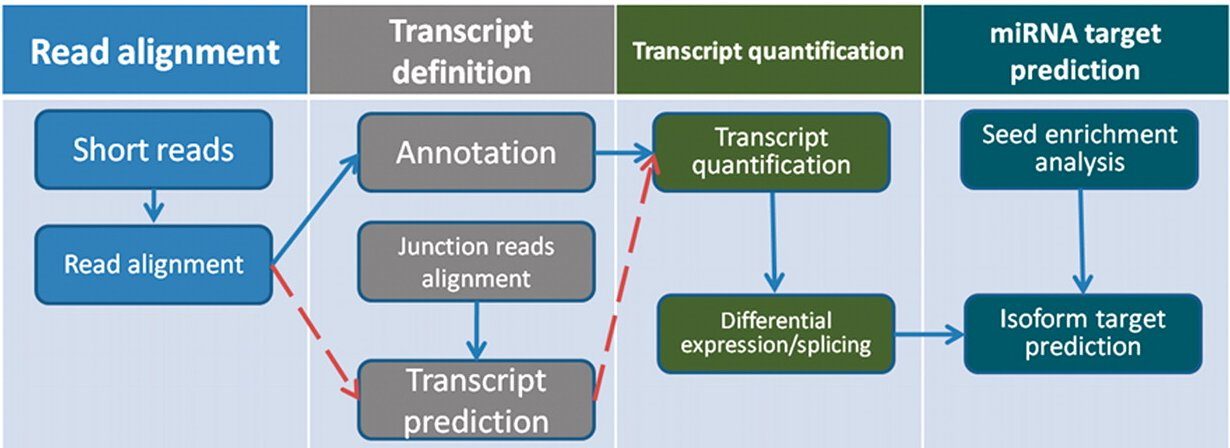
\includegraphics[width=8cm]{c3.workflow.mirna.01.jpg}}
          \item FPKM:Fragments Per Kilobase Million
          \item TPM:Transcripts Per Kilobase Million
          \item RPKM vs. FPKM:SE vs. PE
\parpic[fl]{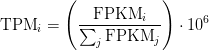
\includegraphics[width=6.5cm,height=1.4cm]{c3.term.tpm.03.png}}
        \end{itemize}
    \end{enumerate}

\otherTail
\newpage
\otherHeader

        \vspace{-1em}
        \begin{figure}[h]
          \centering
          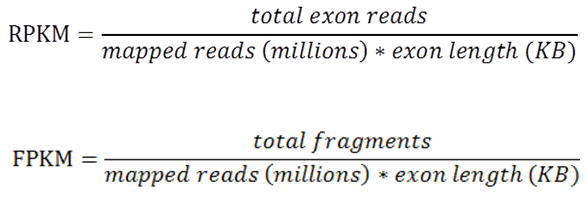
\includegraphics[width=0.5\textwidth]{c3.term.fpkm.03.png}
          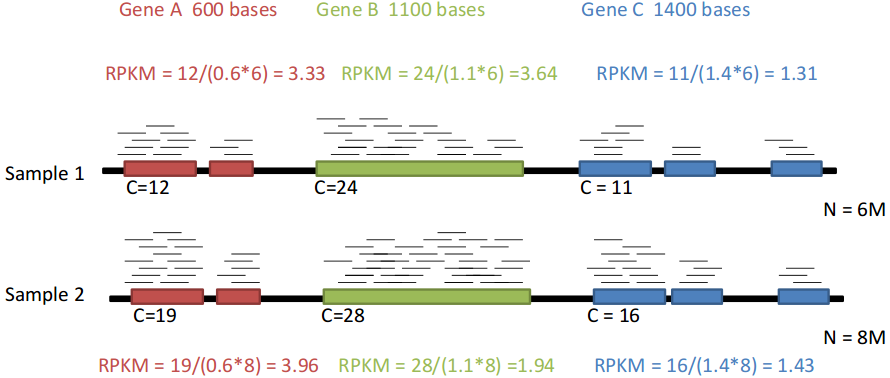
\includegraphics[width=0.45\textwidth]{c3.term.rpkm.03.png}
        \end{figure}
        \vspace{-1em}
        \begin{figure}[h]
          \centering
          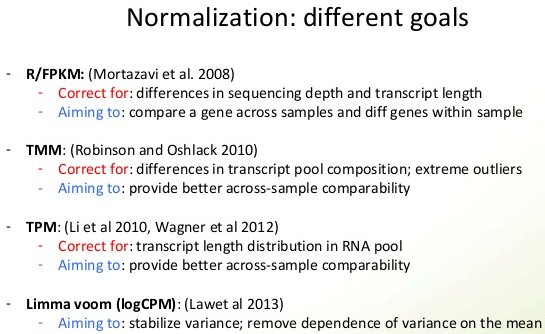
\includegraphics[width=0.5\textwidth]{c3.term.all.02.jpg}
          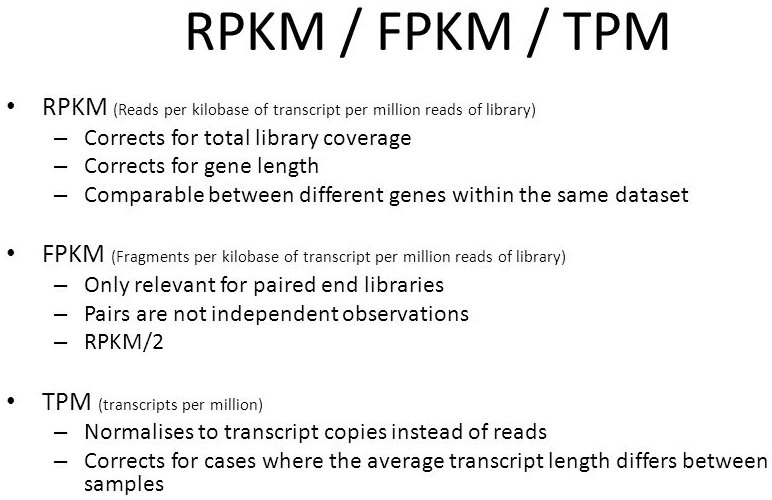
\includegraphics[width=0.45\textwidth]{c3.term.all.04.jpg}
        \end{figure}
        \vspace{-1em}

  \item 总结与答疑(5分钟)
    \begin{enumerate}
      \item 知识点
	\begin{itemize}
	  \item 组学:常见组学
	  \item 转录组学:基本概念,研究内容,研究方法
    \item RNA-Seq:基本概念,常见应用,主要流程,专用术语
	\end{itemize}
      \item 技能
	\begin{itemize}
    \item 掌握RNA-Seq数据分析的基本流程
    \item 掌握RPKM/FPKM/TPM的计算方法
	\end{itemize}
    \end{enumerate}
\end{enumerate}

\otherTail


\end{document}

